\chapter{実験環境}

\section{プログラム}
本実験で使用したプログラムは以下のサイト\cite{semantic_mesh_localization_link}にて公開している. また, 提案手法\cite{semantic_point_localization}はプログラムがインターネット上に公開されていないため論文内のアルゴリズムに従って作成した. 提案手法では画像のスキャンデータから三次元点群地図を生成しているが, 今回の実験においては\ref{sec:dataset}節で詳しく述べるデータセットから直接三次元点群を取得している部分が先行研究の論文内で述べられている実験環境と異なる.

%% PCの仕様
\section{PC}
今回実験では2台の性能の異なるPCを使用した. \ref{sec:result}節で述べる実験結果には動作時間の比較などを除いてPC1を使用したときの結果である. 以下の表\ref{tab:PC_spec}に使用したPCの性能を示す.

\begin{table}[htbp]
\begin{center}
\caption{PCスペック}
  \begin{tabular}{l c c}\hline
       &  PC1 & PC2 \\ \hline
    OS & Ubuntu20.04 LTS & Ubuntu18.04 LTS\\
    CPU & i9-10850K 10core 20thread 3.70GHz & i7-7700 4core 8thread 3.60GHz\\
    GPU & RTX2080Ti 8GB & GTX1060 3GB\\
    RAM & 32GB & 16GB\\ \hline
  \end{tabular}
  \label{tab:PC_spec}
\end{center}
\end{table}

\begin{comment}
\begin{table}[htbp]
\begin{center}
\caption{PC1スペック}
  \begin{tabular}{|l|c|}\hline
    OS & Ubuntu20.04 LTS \\ \hline
    NVIDIA Driver & 460.27.04 \\ \hline
    CPU & Intel Core i9-10850K 10コア 20スレッド 3.70GHz\\ \hline
    GPU & NVIDIA GeForce RTX2080Ti 8GB\\ \hline
    RAM & 32GB \\ \hline
  \end{tabular}
  \label{tab:PC1}
\end{center}
\end{table}

\begin{table}[htbp]
\begin{center}
\caption{PC2スペック}
  \begin{tabular}{|l|c|}\hline
    OS & Ubuntu18.04 LTS \\ \hline
    NVIDIA Driver & 460.27.04 \\ \hline
    CPU & Intel Core i7-7700 4 コア 8 スレッド 3.60GHz\\ \hline
    GPU & NVIDIA GeForce GTX1060 3GB\\ \hline
    RAM & 16GB \\ \hline
  \end{tabular}
  \label{tab:PC2}
\end{center}
\end{table}
\end{comment}


%% UbuntuでROSやTensorRT, PCLのどのバージョンを使いました的なことを書く
\section{ソフトウェア}\label{sec:software}
今回実験においてROSやOpenCV, PCLなどを中心としたソフトウェアを使用した. 表\ref{tab:software}に実験において使用したソフトウェアとそのバージョンを示す.
\begin{table}[htbp]
\begin{center}
\caption{実験に使用したソフトウェア}
  \begin{tabular}{l|c|c|l} \hline
    ソフトウェア名 & バージョン(PC1) & バージョン(PC2) & 備考 \\ \hline
    Robot Operation System & Noetic & Melodic & 以降"ROS"と表記する\\
    Point Cloud Library &1.8.1 & 1.8.1 & 以降"PCL"と表記する\\
    OpenCV & 3.2.0 & 3.2.0 & \\
    Visualization Toolkit & 9.0.1 & 9.0.1 & 以降"VTK"と表記する\\
    yaml-cpp & 0.6.2 & 0.5.2 & \\
    CUDA & 11.2 & 11.1 & \\
    nvinfer & 7.2.1-1 & 7.2.1-1 & \\
    Tensorflow & 2.3.1 & 2.3.1 & \\
    TensorRT & 7.2.1.6-1 & 7.2.1.6-1 & \\ \hline
  \end{tabular}
  \label{tab:software}
\end{center}
\end{table}

%% Semantic KITTIの解説
\section{データセット}\label{sec:dataset}
実験ではボン大学が公表しているSemantic KITTI dataset\cite{semantic_kitti_dataset_paper}\cite{semantic_kitti_dataset_link}を使用した. 本データセットはKITTI Visual Odometry Dataset\cite{Geiger2012CVPR}の点群データに車や建物などセマンティックなラベルを色として付与したPoint Segmentationの精度評価のためのデータセットである. 本データセットは点群にラベルの付いた11の学習用シークエンスとラベルの付いていない実験用の11のシークエンスからなるデータである. シークエンスの中には直線状の道路を10秒間走るだけといったものもあるが, 今回の実験ではそういったシークエンスは使用しない. 今回の実験で使用したシークエンスはsequence00, 02, 05, 08の4つである. それぞれのシークエンスの地図の全体像を図\ref{fig:sequence00}, \ref{fig:sequence02}, \ref{fig:sequence05}, \ref{fig:sequence08}に示す. \par 先行研究\cite{semantic_point_localization}では点群データの存在しないCityScapes Dataset\cite{CityScapes_paper}\cite{CityScapes_link}の画像データから三次元点群を生成して地図を作成していたが,本実験ではラベル付きのデータセットから直接地図を生成する. Semantic KITTI datasetから得られるデータは表\ref{tab:data_from_semantic_kitti}のとおりである. なお, Semantic KITTI datasetにはCityScapesやKITTI dataset\cite{KITTI_dataset_paper}のようにIMUやオドメトリのデータが存在しない. 自己位置推定を行うためには事前分布の更新のためにどちらか, もしくはその両方のデータが必要となる. このため実験では姿勢のGround Truthに正規分布に従う誤差を加えることでオドメトリを再現した. \par 今回ROS上で自己位置推定のためのプログラムを実行する上でこれらのデータセットをROSのbagデータに変換した. 変換に使用したプログラムはGithub上に公開してある\cite{semantickitti2bag}.

\begin{figure}[htbp]
 \begin{minipage}{0.5\hsize}
  \begin{center}
   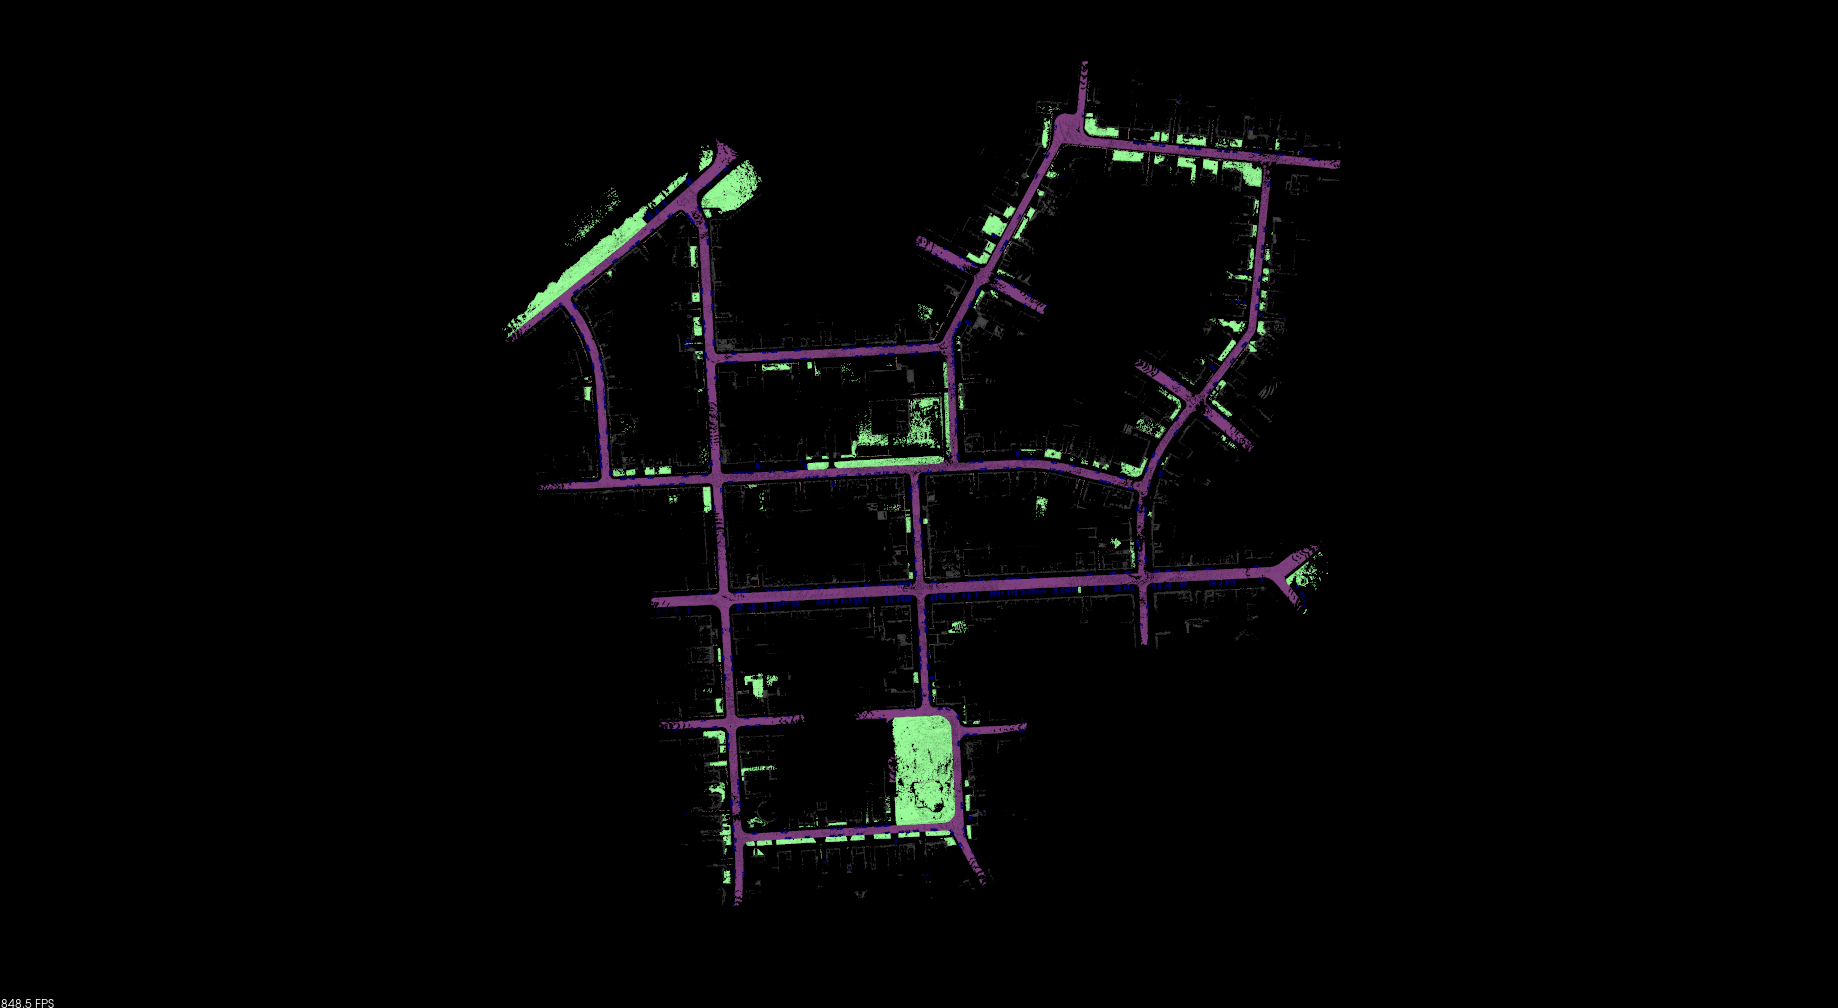
\includegraphics[width=75mm]{./picture/sequence00_map.png}
  \end{center}
  \caption{Sequence00}
  \label{fig:sequence00}
 \end{minipage}
 \begin{minipage}{0.5\hsize}
  \begin{center}
   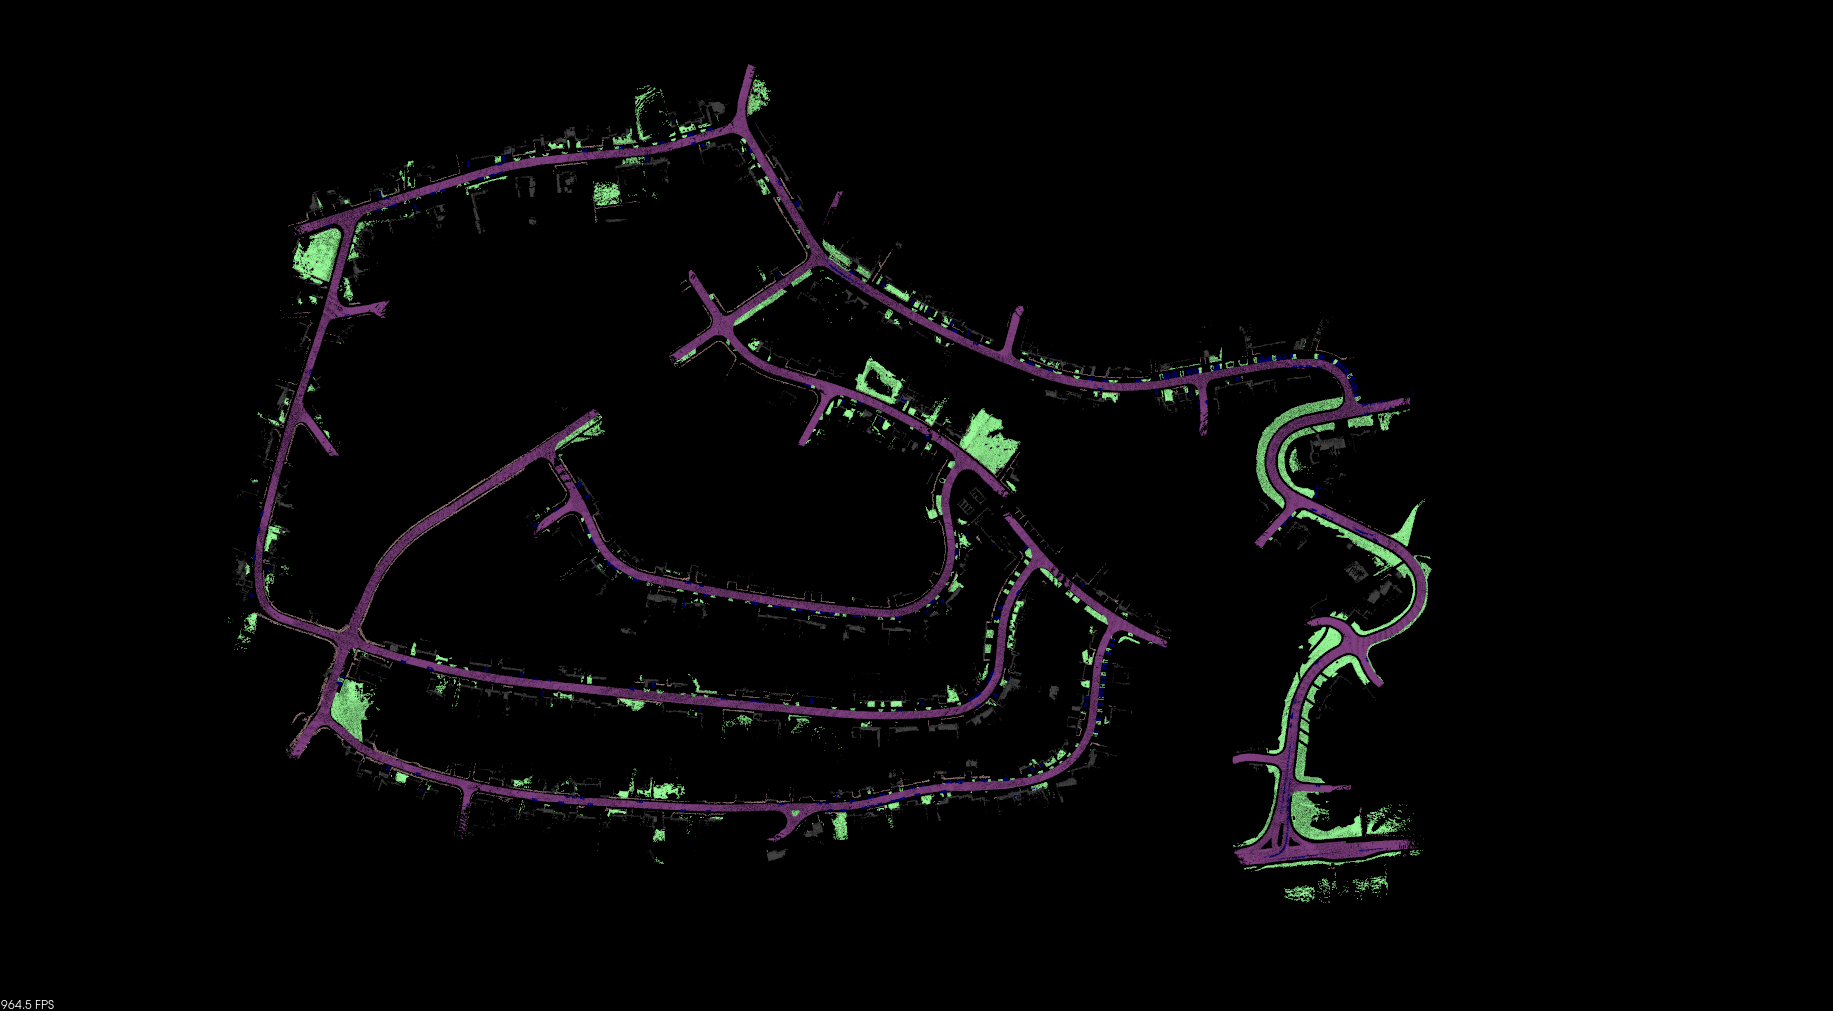
\includegraphics[width=75mm]{./picture/sequence02_map.png}
  \end{center}
  \caption{Sequence02}
  \label{fig:sequence02}
 \end{minipage} \\ \\ \\ \\
  \begin{minipage}{0.5\hsize}
  \begin{center}
   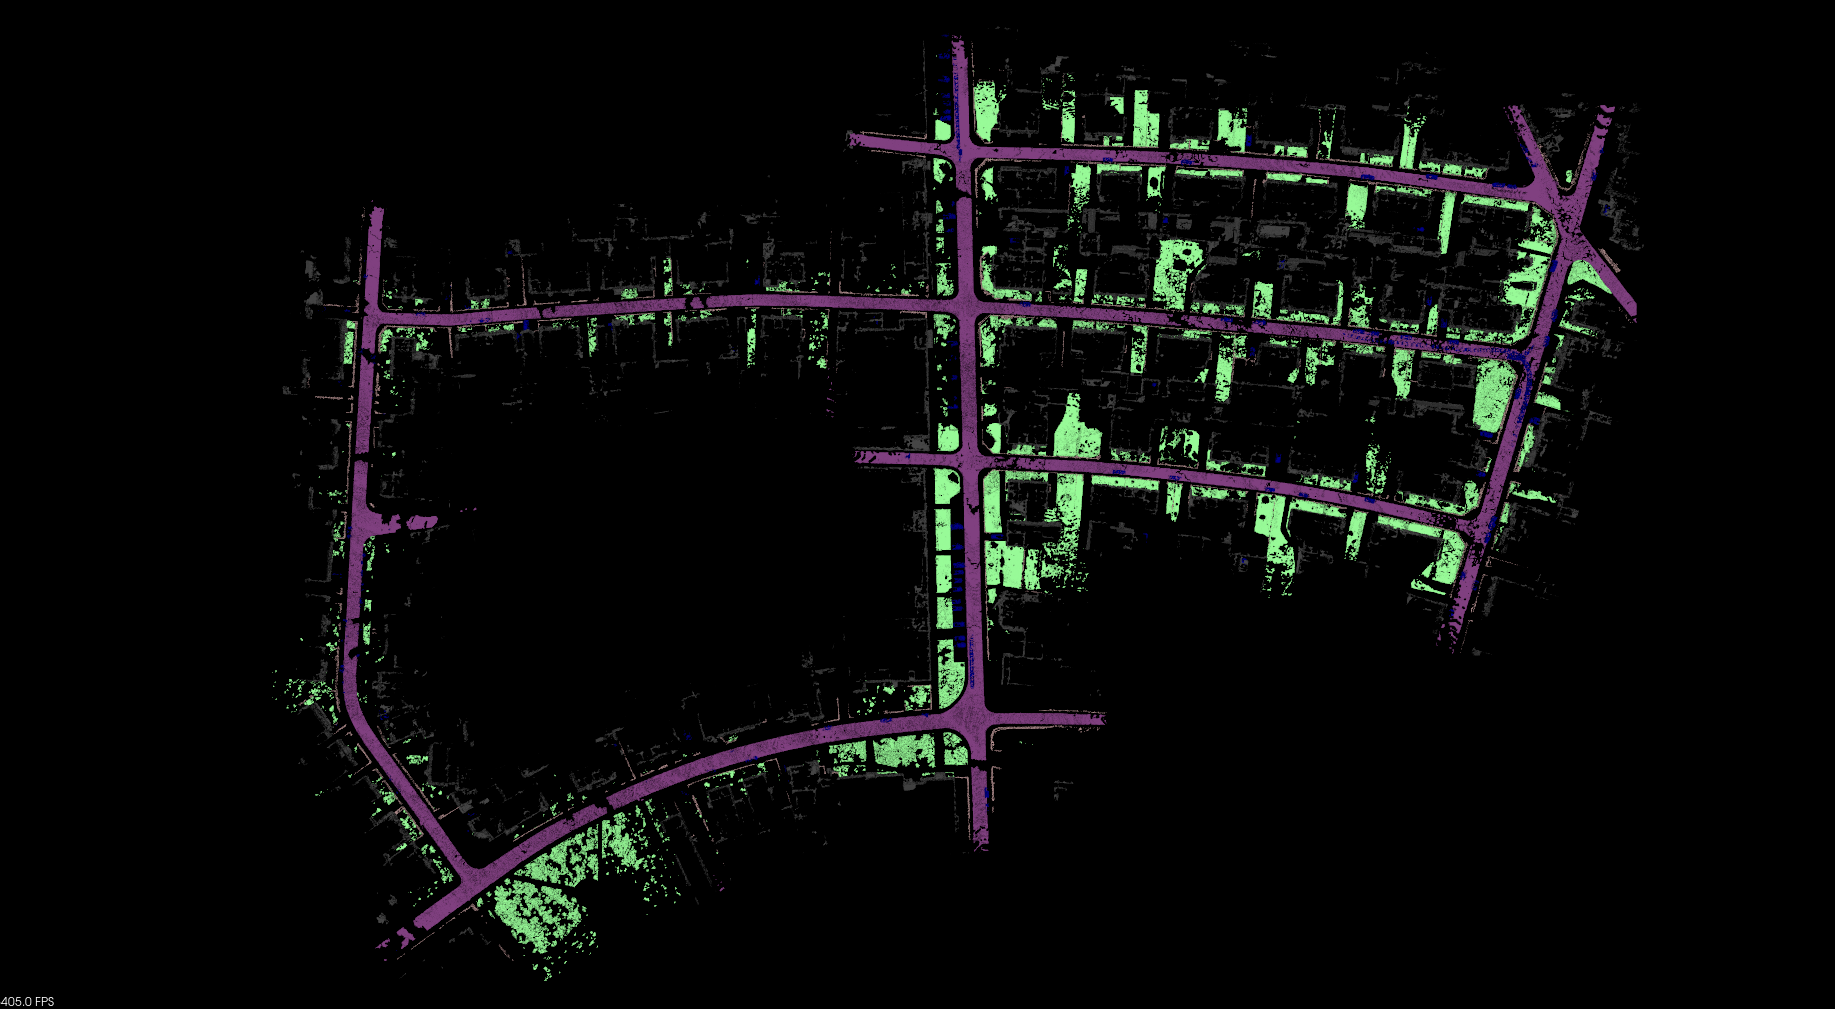
\includegraphics[width=75mm]{./picture/sequence05_map.png}
  \end{center}
  \caption{Sequence05}
  \label{fig:sequence05}
 \end{minipage}
 \begin{minipage}{0.5\hsize}
  \begin{center}
   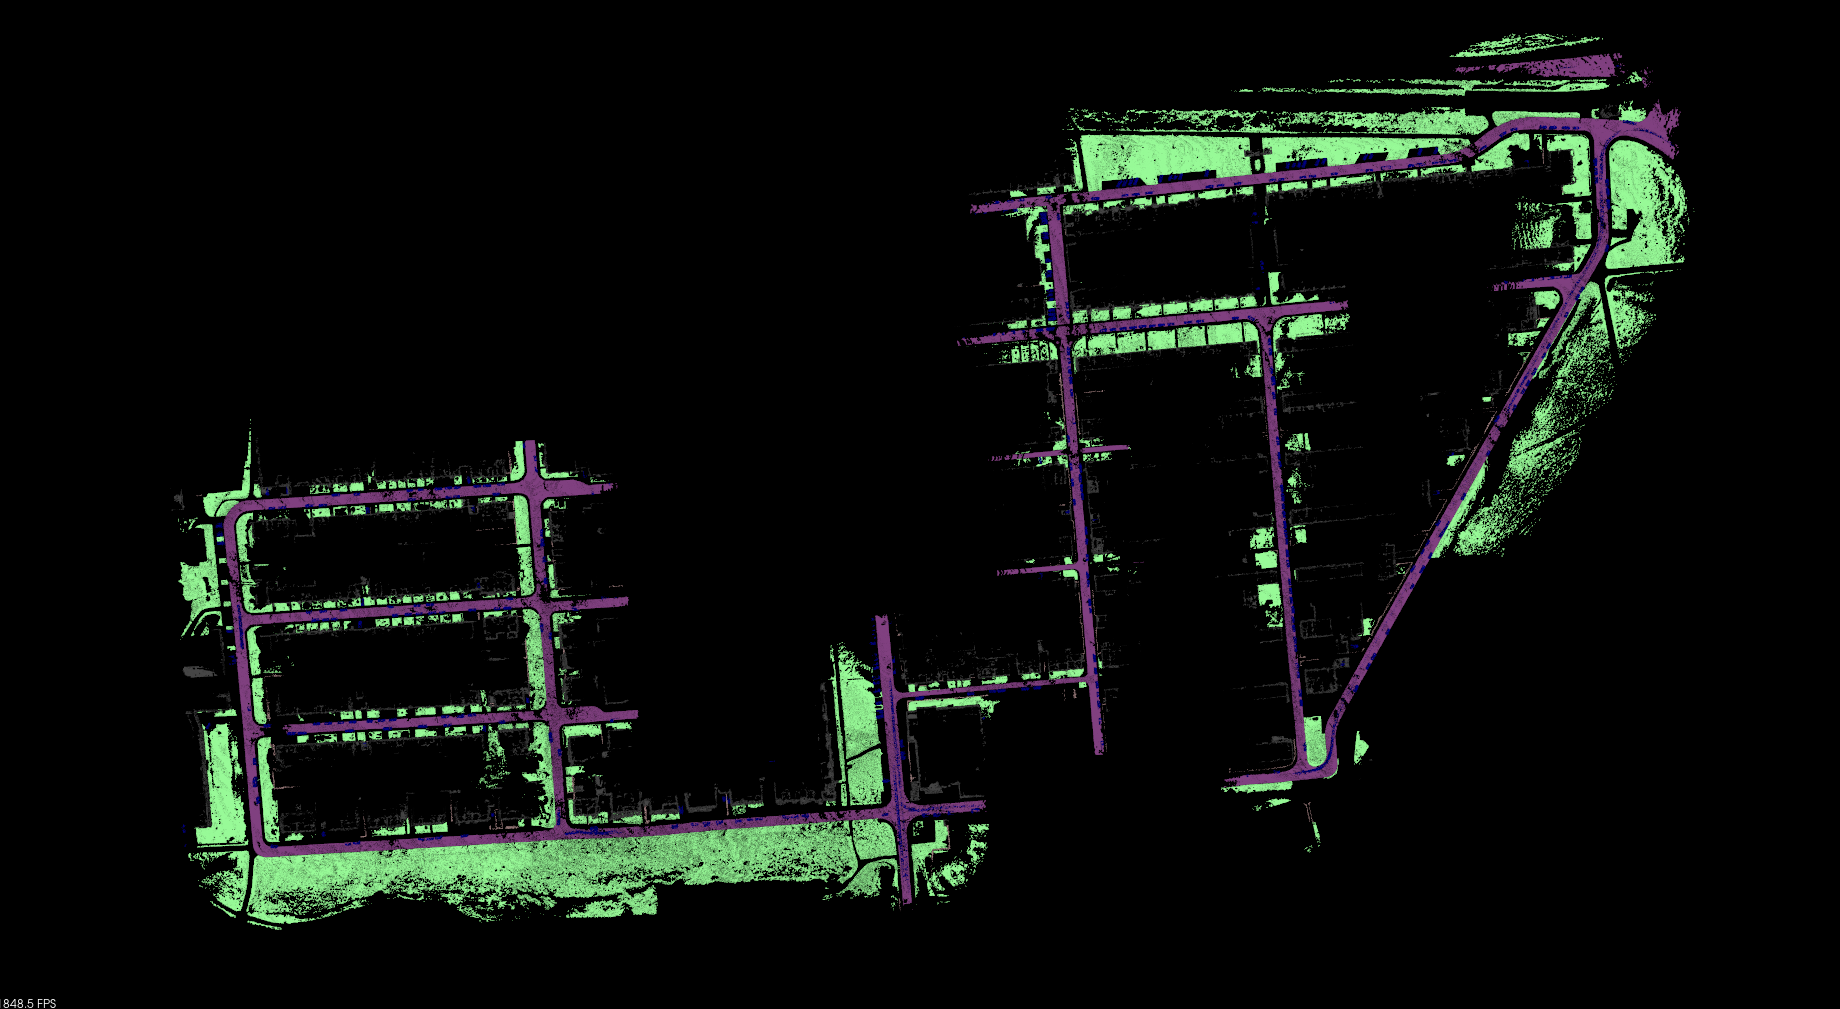
\includegraphics[width=75mm]{./picture/sequence08_map.png}
  \end{center}
  \caption{Sequence08}
  \label{fig:sequence08}
 \end{minipage}
\end{figure}

\begin{table}[htbp]
\begin{center}
\caption{Semantic KITTI dataset から得られるデータ}\label{tab:data_from_semantic_kitti}
  \begin{tabular}{l|l} \hline
    \multicolumn{1}{c|}{データ名} & \multicolumn{1}{c}{備考} \\ \hline
    点群データ & 車や建物などラベルが付与されている \\
    画像データ & 前方に搭載したRGBカメラとモノクロカメラから画像データが得られる \\
    Ground Truth & 精度評価, 及び誤差を含むオドメトリの生成に用いる\\
    固定位置関係 & LiDARとカメラ間の位置関係など時間変化のしない位置関係のデータ \\ \hline
  \end{tabular}
\end{center}
\end{table}

%% odometryの値が真値だからランダムに誤差与えました的なことを書く
%%尤度算出のパラメーターや分散の値を書く
\section{補足}\label{sec:env_appendix}
今回の実験においてモンテカルロ自己位置推定におけるハイパーパラメータを表\ref{tab:MCL_parameter}, 尤度算出におけるハイパーパラメータを表\ref{tab:likelihood_parameter}に示す. また, 表\ref{tab:likelihood_parameter}の値はAlg.\ref{alg:calc_likelihood}における関数semantic score()の出力値である.

\begin{table}[htbp]
\begin{center}
\caption{メッシュ地図での自己位置推定におけるハイパーパラメータ}
  \begin{tabular}{l|r|l} \hline
    \multicolumn{1}{c|}{パラメータ名} & \multicolumn{1}{c|}{値} & \multicolumn{1}{c}{役割} \\ \hline
    BiasXY & 0.030 & 正規分布に従うオドメトリのXY方向の誤差の分散 \\
    BiasZ & 0.020 & 正規分布に従うオドメトリのZ方向の誤差の分散 \\
    BiasRPY & 0.020 & 正規分布に従うオドメトリのRPY方向の誤差の分散 \\
    XDev & 0.300 & 正規分布に従って広がるパーティクルのX方向の分散 \\
    YDev & 0.300 & 正規分布に従って広がるパーティクルのY方向の分散 \\
    ZDev & 0.130 & 正規分布に従って広がるパーティクルのZ方向の分散 \\
    RollDev & 0.015 & 正規分布に従って広がるパーティクルのRoll方向の分散 \\
    PitchDev & 0.015 & 正規分布に従って広がるパーティクルのPitch方向の分散 \\
    YawDev & 0.015 & 正規分布に従って広がるパーティクルのYaw方向の分散 \\
    ImageDownWidth & 0.250 & カメラ画像のサイズ変更の比率, 処理軽減のため \\
    ImageDownHeight & 0.250 & カメラ画像のサイズ変更の比率, 処理軽減のため \\
    ParticleNumber & 100 & モンテカルロ自己位置推定におけるパーティクルの数 \\
    Averagenumber & 5 & \ref{sec:estimate_current_pose}節の処理にて上位何個のパーティクルの平均を取るか \\ \hline
  \end{tabular}
  \label{tab:MCL_parameter}
\end{center}
\end{table}

\begin{table}[htbp]
\begin{center}
\caption{尤度算出におけるハイパーパラメータ}
  \begin{tabular}{l c l} \hline
    クラス & 値 & 補足\\ \hline
    Road & 0.7 & \\
    Sidewalk & 1.5 & \\
    Car & 4.0 & \\
    Building & 0.7 & \\
    Terrain & 2.0 & 芝生を指す\\
    Other Class & 1.0 & \\ \hline
  \end{tabular}
  \label{tab:likelihood_parameter}
\end{center}
\end{table}
